%!TEX root = chi14grammatical.tex
A list of phrases is the most recognizable presentation for clausal relationships, and is as good as a list of words for the other types of relations. This implies that auto-suggest interfaces for syntactic search should use this format. A mockup of such a search box is shown in Figure \ref{fig:phrases-mockup}.
\begin{figure}
\centering
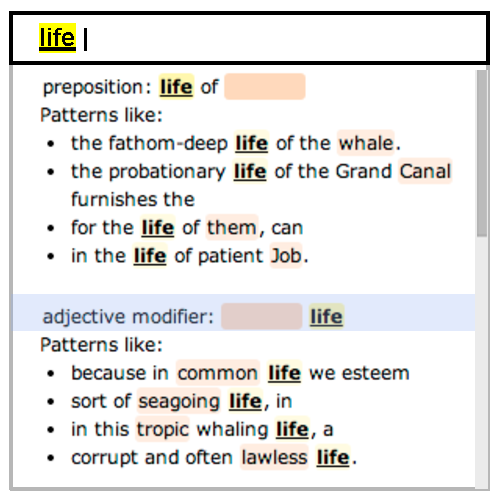
\includegraphics[width=0.5\columnwidth]{fig/phrases-mockup}
\caption{
	\label{fig:phrases-mockup} Mockup of auto-suggest for syntactic search on the word `life', showing the most common grammatical relations with example phrases for each.
}
\end{figure}

\subsection{Future Work}
While \strong{phrases} were slightly better than \strong{words} overall for the non-clausal relations (Figure \ref{fig:results-by-relation-type}), there was one relation for which the opposite seemed to be true. For adverb modifiers (\code{advmod}) (Figure \ref{fig:advmod}), the data seemed to suggest that \strong{words} (0.63\% success) made the relation more recognizable than \strong{phrases} (0.47\% success, $p = 0.055$), which is barely significant due to the smaller sample size (only 96 participants encountered this relation).
